\chapter{Metodologia}

\section{Problema direto}

Seja $\mathbf{d}^{o}$ o vetor de dados observados, cujo $i$-ésimo elemento $d^{o}_{i}$, $i = 1, \dots, N$, é a anomalia de campo total observada (Equação \ref{eq:tfanomaly-general}) no ponto $(x_{i}, y_{i}, z_{i})$.
Considere que as anomalias de campo total produzidas por pequenas fontes magnéticas não-alvo podem distorcer localmente a anomalia causada por uma fonte alvo 3D.
Adicionalmente considere que o campo geomagnético principal é constante na área de estudo, com declinação $ D_ {0} $ e inclinação $ I_ {0} $.
Este trabalho segue a mesma abordagem apresentada por \cite{oliveirajr_etal2011} e \cite{oliveirajr_barbosa2013} para definir o modelo interpretativo que aproxima a geometria da fonte alvo.
Esse modelo é formado por um conjunto de $L$ prismas retos verticalmente justapostos tendo a mesma espessura $dz$ e o mesmo vetor de magnetização total com intensidade $m_{0}$, declinação $D$ e inclinação $I$ (Figura \ref{fig:schematic}).

A profundidade do topo do prisma mais raso é definida por $z_{0}$.
Cada prisma possui a seção horizontal definida por um polígono com $V$ vértices igualmente espaçados de $0^{\circ}$ a $360^{\circ}$.
As posições horizontais dos vértices que formam o $k$-ésimo prisma
são definidas por distâncias radiais (ou apenas raios) $r^{k}_{j}$, com respeito a uma origem $(x_{0}^{k}, y_{0}^{k})$ localizada dentro do prisma, $k = 1, \dots, L$, $j = 1, \dots, V$ (Figura \ref{fig:pk}).
A anomalia de campo total predita pelo modelo interpretativo no ponto $(x_{i}, y_{i}, z_{i})$, $i = 1, \dots, N$, é dada por:
\begin{equation}
d_{i} (\mathbf{p}) \equiv \sum\limits_{k=1}^{L} f_{i}^{k}(\mathbf{r}^{k}, x_{0}^{k}, y_{0}^{k}, dz, z_{1}^{k}, m_{0}, D, I, D_{0}, I_{0}) \: ,
\label{eq:predicted-data-i}
\end{equation}
em que $\mathbf{r}^{k}$ é um vetor de dimensão $V \times 1$ que contém os raios $r^{k}_{j}$ dos vértices pertencentes ao $k$-ésimo prisma, que possui origem no ponto $(x_{0}^{k}, y_{0}^{k})$ e profundidade do topo em $z_{1}^{k} = z_{0} + (k-1)dz$.
Na Equação \ref{eq:predicted-data-i}, $\mathbf{p}$ é um vetor de parâmetros de dimensão $M \times 1$, $ M=L(V+2) +1 $, que define a geometria do modelo interpretativo:
%\begin{equation}
%\mathbf{p} = \left[ \begin{array}{@{}*{12}{c}@{}}
%{\mathbf{r}^{1}}^{\mathsf{T}} & x_{0}^{1} & y_{0}^{1} & \dots & {\mathbf{r}^{L}}^{\mathsf{T}} & x_{0}^{L} & y_{0}^{L} & dz \\
%\end{array} \right]^{\mathsf{T}} \: .
%\label{eq:p-vector}
%\end{equation}
\begin{equation}
\mathbf{p} = \begin{bmatrix} 
{\mathbf{r}^{1}}^{\top} & x_{0}^{1} & y_{0}^{1} & \dots & 
{\mathbf{r}^{L}}^{\top} & x_{0}^{L} & y_{0}^{L} & dz
\end{bmatrix}^{\top} \: .
\label{eq:p-vector}
\end{equation}
A anomalia de campo total $d_{i} (\mathbf{p})$ 
(Equação \ref{eq:predicted-data-i}) é computada por meio das fórmulas de \cite{plouff1976} implementadas no pacote de Python 
Fatiando a Terra \citep{uieda-etal2013}.

%FIGURA
\begin{figure}[!htb]
	\centering
	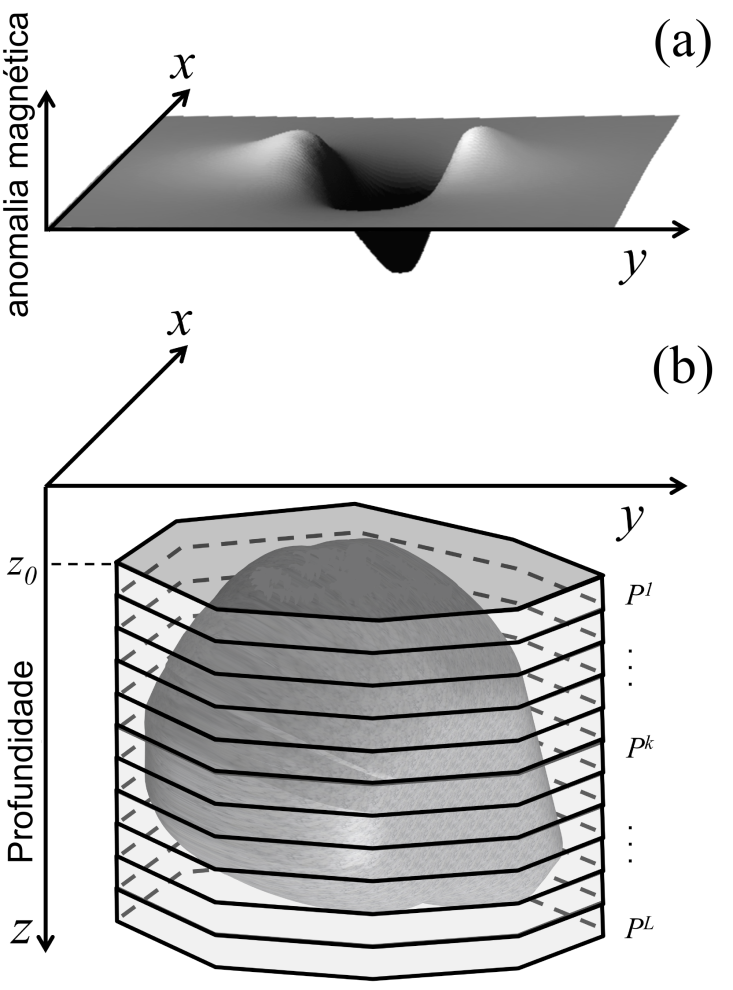
\includegraphics[scale=0.35]{schematic.png}
	\caption{Representação esquemática do modelo interpretativo. (a) Anomalia de campo total produzida por uma fonte magnética 3D localizada em subsuperfície (volume cinza escuro em b). (b) Modelo interpretativo formado por $ L $ prismas retos, verticalmente justapostos e com seção horizontal descrita por um polígono. A profundidade do topo $z_0$ do modelo interpretativo coincide com a da fonte magnética (volume cinza escuro).}
	\label{fig:schematic}
\end{figure}

%FIGURA
\begin{figure}[!htb]
	\centering
	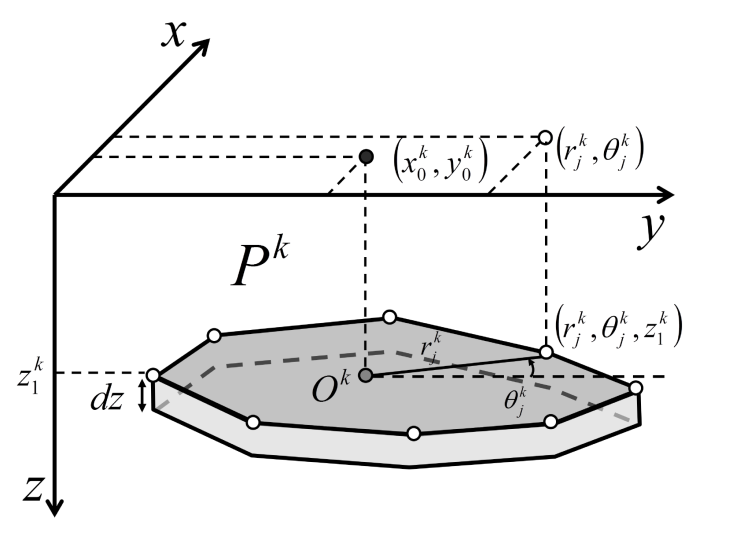
\includegraphics[scale=0.45]{pk.png}
	\caption{Representação esquemática do $k$-ésimo prisma $P^k$, $k=1,\dots, L$, que compõe o modelo interpretativo (Figura 1b). Este prisma tem espessura dz, profundidade do topo $z_1^k$ e seção horizontal descrita por um polígono com $V$ vértices igualmente espaçados entre $0^{\circ}$ e $360^{\circ}$.
}
	\label{fig:pk}
\end{figure}
\pagebreak

\section{Problema inverso}

Este trabalho propõe um método robusto de inversão magnética para estimar a posição e a forma de uma fonte magnética alvo 3D, que pode ou não estar na presença de fontes não-alvo.
O método foi formulado como um problema de otimização não-linear vinculado para estimar um vetor de parâmetros $\mathbf{p}$ (Equação \ref{eq:p-vector}) minimizando a função objetivo
\begin{equation}
\Gamma (\mathbf{p}) = \phi (\mathbf{p}) + \sum\limits^{5}_{\ell =1} \alpha_{\ell} \, \varphi_{\ell}(\mathbf{p}) \: ,
\label{eq:gamma}
\end{equation}
sujeito aos vínculos de desigualdade
\begin{equation}
p_{l}^{min} < p_{l} < p_{l}^{max}, \quad l = 1, \dots, M \: ,
\label{eq:inequality-constraints}
\end{equation}
em que $p_{l}^{min}$ e $p_{l}^{max}$ definem, respectivamente, os limites inferior e superior para o $l$-ésimo elemento $p_{l}$ do vetor de parâmetros $\mathbf{p}$,
$\varphi_{\ell}(\mathbf{p})$ são as funções que representam os vínculos que impõem informação a priori sobre a forma da estimativa do corpo 3D, e $\phi (\mathbf{p})$ 
é a função desajuste dos dados -- ou \textit{data-misfit} em inglês.
Podemos definir $\phi (\mathbf{p})$ através de duas abordagens diferentes com o propósito de comparar os resultados. Na primeira abordagem, $\phi (\mathbf{p})$ como
\begin{equation}\label{eq:L2_misfit}
\phi (\mathbf{p}) = \frac{1}{N} 
\| \mathbf{d}^{o} - \mathbf{d}(\mathbf{p}) \|_{2}^{2} \quad ,
\end{equation}
que é a norma-2 quadrática \citep[por exemplo,][p. 331]{aster_etal2019} dos resíduos entre o vetor de dados observados $\mathbf{d}^{o}$, cujo $i$-ésimo elemento $d_{i}^{o}$ representa a anomalia de campo total observada no ponto $(x_{i}, y_{i}, z_{i})$, e o vetor de dados preditos $\mathbf{d}(\mathbf{p})$, cujo $i$-ésimo elemento $d_{i} (\mathbf{p})$ é definido pela Equação \ref{eq:predicted-data-i}.
Alternativamente, podemos definir a função \textit{data-misfit} como
\begin{equation}\label{eq:L1_misfit}
\phi (\mathbf{p}) = \frac{1}{N} 
\| \mathbf{d}^{o} - \mathbf{d}(\mathbf{p}) \|_{1} \quad ,
\end{equation}
que representa a norma-1 \citep[por exemplo,][p. 331]{aster_etal2019}
dos resíduos entre os vetores de dados observados $\mathbf{d}^{o}$ e preditos $\mathbf{d}(\mathbf{p})$.
É de amplo conhecimento que o vetor de parâmetros que minimiza a norma-2 quadrática (Equação \ref{eq:L2_misfit}) pode ser muito afetado negativamente pela presença de \textit{outliers} e também pelo efeito causado por fontes não-alvo \cite[por exemplo,][]{claerbout_muir1973, 
	silva_hohmann1983, scales_gersztenkorn1988, silva_cutrim1989, farquharson_oldenburg1998, 
	uieda_barbosa2012, oliveirajr_etal2015, aster_etal2019}.
Através da estimativa do vetor de parâmetros obtida pela minimização da norma-1 (Equação \ref{eq:L1_misfit}), espera-se que a posição e a forma estimadas do corpo 3D durante a inversão ajustem a anomalia de campo total produzida pela fonte alvo e ignorem a causada pelas fontes não-alvo.

Na Equação \ref{eq:gamma}, $\alpha_{\ell}$, $\ell = 1, \dots, 5$, são escalares positivos que definem o peso relativo das funções dos vínculos $\varphi_{\ell}(\mathbf{p})$.
Essas funções são definidas seguindo a mesma abordagem utilizada por \citet{oliveirajr_etal2011} e \citet{oliveirajr_barbosa2013}.

\section{Vínculos}\label{sec:constraints}

As funções dos vínculos $\varphi_{\ell}(\mathbf{p})$ (Equação \ref{eq:gamma}), $\ell = 1, \dots, 5$, utilizadas aqui para obter soluções estáveis e introduzir informação a priori sobre o corpo estimado, foram organizadas em dois grupos para um melhor entendimento.

\subsection{Vínculos de suavidade}

Este grupo é formado pelas variações da regularização de Tikhonov de primeira ordem \cite[][ p. 103]{aster_etal2019} que impõe suavidade sobre os raios $r_{j}^{k}$ e sobre as coordenadas Cartesianas $x_{0}^{k}$ e $y_{0}^{k}$ da origem $O^{k}$, $j = 1, \dots, V$, $k = 1, \dots, L$, que define a seção horizontal de cada prisma (Fig.\ref{fig:schematic}b).
Elas foram propostas por \cite{oliveirajr_etal2011} e \cite{oliveirajr_barbosa2013} e possuem um papel muito importante em introduzir informação a priori sobre a forma da fonte alvo. 

O primeiro vínculo deste grupo é a \textit{suavidade sobre os raios adjacentes que definem a seção horizontal de cada prisma}. Esse vínculo impõe que os raios adjacentes $r_{j}^{k}$ e $r_{j+1}^{k}$ dentro do mesmo prisma devem ter comprimento semelhantes. Isso força que o prisma estimado terá uma forma aproximadamente cilíndrica, que evita descontinuidades abruptas entre as estimativas das distâncias radiais dentro de um mesmo prisma. Sua representação esquemática é mostrada na Figura \ref{fig:phi1}.

%FIGURA
\begin{figure}[!htb]
	\centering
	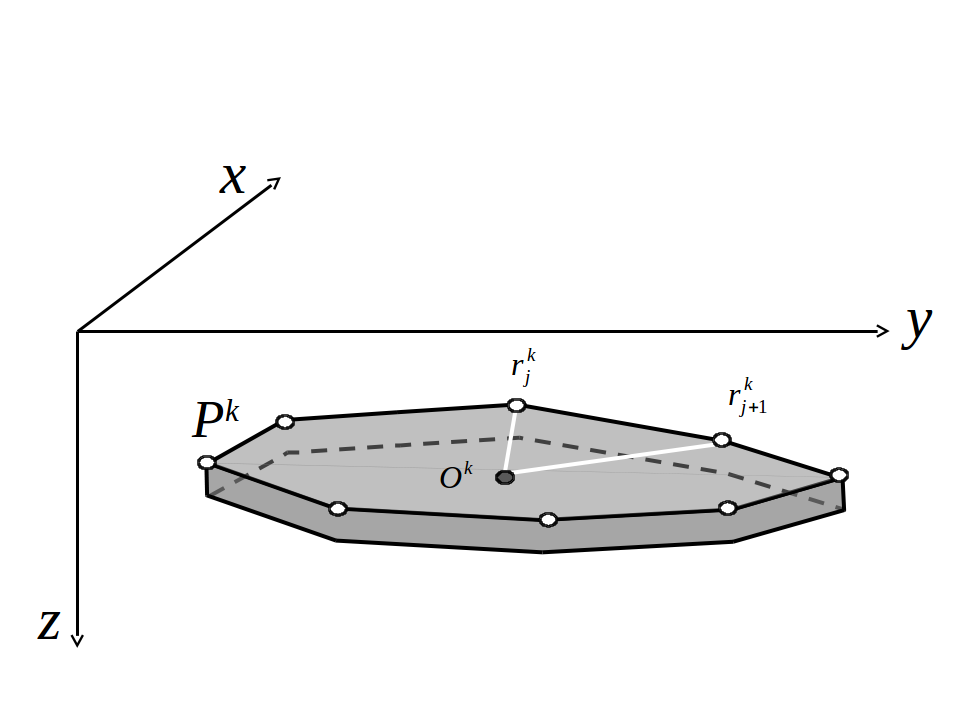
\includegraphics[scale=0.45]{Constraint_phi1.png}
	\caption{Representação esquemática do vínculo de suavidade sobre distâncias adjacentes dentro de um mesmo prisma $\varphi_{1}$. A figura exibe o k-ésimo prisma $P^k$ e as distâncias radiais adjacentes $r_j^k$ e $r_{j+1}^k$ relacionadas ao vínculo.}
	\label{fig:phi1}
\end{figure}

Matematicamente, o vínculo é dado por \begin{equation}\label{eq:phi1}
\begin{split}
\varphi_{1}(\mathbf{p}) &= \sum\limits^{L}_{k=1}\left[\left(r^{k}_{V}-r^{k}_{1}\right)^2 + \sum\limits^{V-1}_{j=1}\left(r^{k}_{j}-r^{k}_{j+1}\right)^2\right]\\
&= \mathbf{p}^{\mathsf{T}} \mathbf{R}^{\mathsf{T}}_{1}\mathbf{R}_{1} \mathbf{p} \quad ,
\end{split}
\end{equation}
em que
\begin{equation}
\mathbf{R}_{1} = 
\mathbf{I}_{L} \otimes 
\begin{bmatrix}
\left( \mathbf{I}_{V} - \mathbf{D}_{V}^\mathsf{T} \right) & \mathbf{0}_{V \times 2} \\
\end{bmatrix}_{LV \times M} \quad ,
\label{eq:S1-matrix}
\end{equation}
$\mathbf{I}_{L}$ é a matriz identidade de ordem $L$, ``$\otimes$" indica o produto de Kronecker \cite{}\cite[][ p. 243]{horn_johnson1991}, $\mathbf{0}_{V \times 2}$ é uma matriz de ordem $V \times 2$ com elementos nulos, 
$\mathbf{I}_{V}$ é a matriz identidade de ordem $V$ e $\mathbf{D}_{V}^\mathsf{T}$ é a matriz de permutação superior de ordem $V$ \cite[][ p. 20]{golub-vanloan2013}. O vetor gradiente e a matriz Hessiana da função $\varphi_{1}(\mathbf{p})$ (Equação \ref{eq:phi1}) são dados por:
\begin{equation}\label{eq:phi1_gh}
\begin{split}
\boldsymbol{\nabla}\varphi_{1}(\mathbf{p}) &= 2 \mathbf{R}^\mathsf{T}_{1}\mathbf{R}_{1}\mathbf{p} \quad , \\
\mathbf{H}_{1}(\mathbf{p}) &= 2\mathbf{R}^\mathsf{T}_{1}\mathbf{R}_{1} \quad .
\end{split}
\end{equation}

O segundo vínculo do grupo é a \textit{suavidade sobre os raios adjacentes de prismas adjacentes}, o qual impõe que os raios adjacentes $r_{j}^{k}$ e $r_{j}^{k+1}$ entre prismas verticalmente adjacentes tenham comprimentos semelhantes. Esse vínculo força que a forma de prismas verticalmente adjacentes seja similar. Uma representação esquemática do vínculo é apresentada na Figura \ref{fig:phi2}.

%FIGURA
\begin{figure}[!htb]
	\centering
	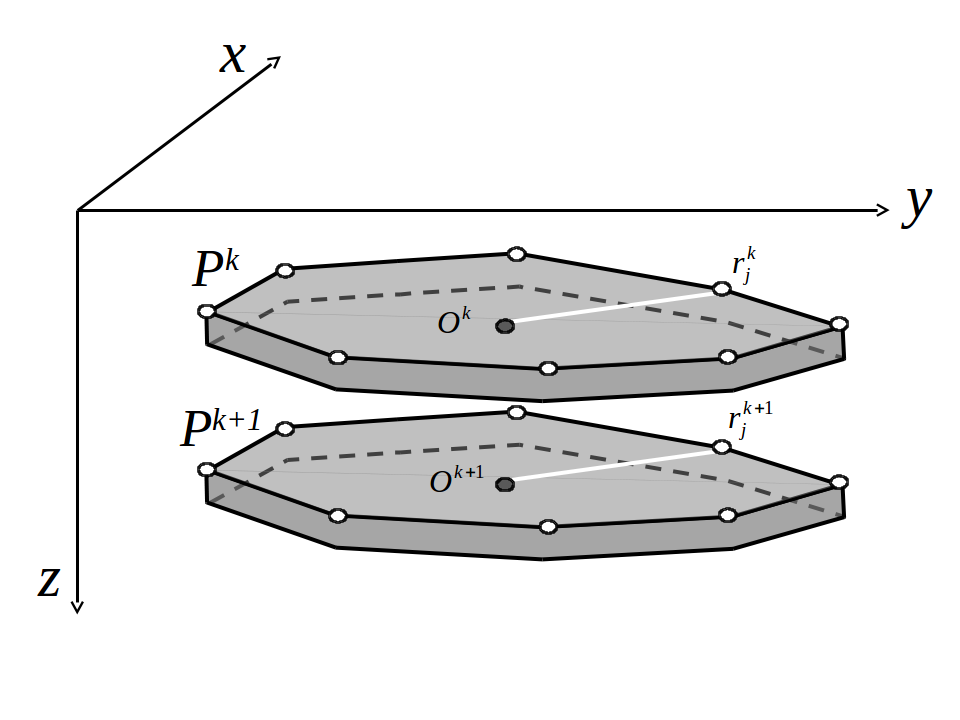
\includegraphics[scale=0.45]{Constraint_phi2.png}
	\caption{Representação esquemática do vínculo de suavidade sobre distâncias adjacentes pertencentes a prismas adjacentes $\varphi_{2}$. A figura exibe o k-ésimo prisma $P^k$ e seu adjacente $P^{k+1}$, assim como as distâncias radiais adjacentes $r_j^k$ e $r_j^{k+1}$ relacionadas ao vínculo.}
	\label{fig:phi2}
\end{figure}

De forma matemática o vínculo é dado por
\begin{equation}\label{eq:phi2}
\begin{split}
\varphi_{2}(\mathbf{p}) &= \sum\limits^{L-1}_{k=1}\left[\sum\limits^{V}_{j=1}\left(r^{k+1}_{j}-r^{k}_{j}\right)^2\right] \\
&= \mathbf{p}^{\mathsf{T}} \mathbf{R}^{\mathsf{T}}_{2}\mathbf{R}_{2}\mathbf{p}
\end{split} \quad ,
\end{equation}
em que
\begin{equation}
\mathbf{R}_{2} = 
\begin{bmatrix}
\mathbf{S}_{2} & \mathbf{0}_{(L-1)V \times 1} \\
\end{bmatrix}_{(L-1)V \times M} \quad ,
\label{eq:R2-matrix}
\end{equation}
\begin{equation}
\mathbf{S}_{2} =
\left( 
\begin{bmatrix} \mathbf{I}_{L-1} & \mathbf{0}_{(L-1) \times 1} \end{bmatrix} -
\begin{bmatrix} \mathbf{0}_{(L-1) \times 1} & \mathbf{I}_{L-1} \end{bmatrix} 
\right) \otimes 
\begin{bmatrix} \mathbf{I}_{V} & \mathbf{0}_{V \times 2} \end{bmatrix} \quad ,
\label{eq:S2-matrix}
\end{equation}
$\mathbf{0}_{(L-1)V \times 1}$ é um vetor de ordem $(L-1)V \times 1$ com elementos nulos,
$\mathbf{0}_{(L-1) \times 1}$ é um vetor de ordem $(L-1) \times 1$ com elementos nulos e 
$\mathbf{I}_{L-1}$ é a matriz identidade de ordem $L-1$. O vetor gradiente e a matriz Hessiana da função $\varphi_{2}(\mathbf{p})$ (Equação \ref{eq:phi2}) são dados por:
\begin{equation}\label{eq:phi2_gh}
\begin{split}
\boldsymbol{\nabla}\varphi_{2}(\mathbf{p}) &= 2\mathbf{R}^\mathsf{T}_{2}\mathbf{R}_{2}\mathbf{p} \quad ,\\
\mathbf{H}_{2}(\mathbf{p}) &= 2\mathbf{R}^\mathsf{T}_{2}\mathbf{R}_{2} \quad .
\end{split}
\end{equation}

O último vínculo deste grupo é a \textit{suavidade sobre a posição horizontal das origens arbitrárias de prismas verticalmente adjacentes}. Esse vínculo impõe que as coordenadas Cartesianas horizontais estimadas $(x_{0}^{k}, y_{0}^{k})$ e $(x_{0}^{k+1}, y_{0}^{k+1})$ das origens $O^{k}$ e $O^{k+1}$ 
de prismas verticalmente adjacentes devem ser próximas entre si. Isso controla o mergulho do corpo estimado através da regularização do deslocamento horizontal de prismas verticalmente adjacentes (Figura \ref{fig:phi3}).

%FIGURA
\begin{figure}[!htb]
	\centering
	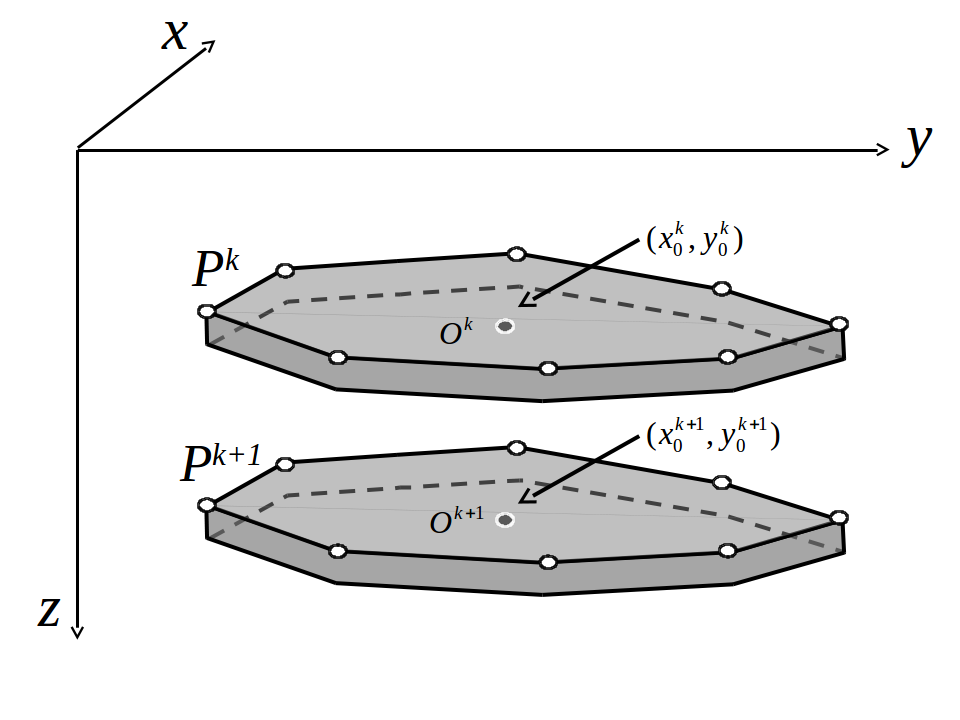
\includegraphics[scale=0.45]{Constraint_phi5.png}
	\caption{Representação esquemática do vínculo de suavidade nas coordenadas das origens pertencentes a prismas adjacentes $\varphi_{3}$. A figura exibe os prismas $P^k$ e $P^{k+1}$ e suas respectivas as coordenadas Cartesianas $(x_0^k,y_0^k)$, referidas à origem $O^k$, e $(x_0^{k+1},y_0^{k+1})$, referidas à origem $O^{k+1}$.}
	\label{fig:phi3}
\end{figure}

Algebricamente o vínculo é dado por
\begin{equation}\label{eq:phi3}
\begin{split}
\varphi_{3}(\mathbf{p}) &= \sum\limits^{L-1}_{k=1}\left[\left(x_{0}^{k+1} - x_{0}^{k}\right)^2 + \left(y_{0}^{k+1} - y_{0}^{k}\right)^2 \right] \\
&= \mathbf{p}^{\mathsf{T}} \mathbf{R}^{\mathsf{T}}_{3}\mathbf{R}_{3}\mathbf{p}
\end{split} \quad ,
\end{equation}
em que 
\begin{equation}
\mathbf{R}_{3} = 
\begin{bmatrix}
\mathbf{S}_{3} & \mathbf{0}_{(L-1)2 \times 1} \\
\end{bmatrix}_{(L-1)2 \times M} \quad ,
\label{eq:R3-matrix}
\end{equation}
\begin{equation}
\mathbf{S}_{3} =
\left( 
\begin{bmatrix} \mathbf{I}_{L-1} & \mathbf{0}_{(L-1) \times 1} \end{bmatrix} -
\begin{bmatrix} \mathbf{0}_{(L-1) \times 1} & \mathbf{I}_{L-1} \end{bmatrix} 
\right) \otimes 
\begin{bmatrix} \mathbf{0}_{2 \times V} & \mathbf{I}_{2} \end{bmatrix} \quad ,
\label{eq:S3-matrix}
\end{equation}
$\mathbf{0}_{(L-1)2 \times 1}$ é um vetor de ordem $(L-1)2 \times 1$ com elementos nulos,
$\mathbf{0}_{2 \times V}$ é uma matrix de ordem $2 \times V$ com elementos nulos e 
$\mathbf{I}_{2}$ é uma matriz identidade de ordem $2$. O vetor gradiente e a matriz Hessiana da função $\varphi_{3}(\mathbf{p})$ (Equação \ref{eq:phi3}) são dados por:
\begin{equation}\label{eq:phi3_gh}
\begin{split}
\boldsymbol{\nabla}\varphi_{3}(\mathbf{p}) &= 2\mathbf{R}^\mathsf{T}_{3}\mathbf{R}_{3}\mathbf{p} \quad ,\\
\mathbf{H}_{3}(\mathbf{p}) &= 2\mathbf{R}^\mathsf{T}_{3}\mathbf{R}_{3} \quad .
\end{split}
\end{equation}

\subsection{Vínculos de norma Euclidiana mínima}

Dois vínculos utilizam a regularização Tikhonov de ordem zero com o propósito de estabilizar de maneira puramente matemática o problema inverso sem necessariamente introduzir informação a priori com significado físico sobre a fonte. 

A \textit{norma Euclidiana mínima dos raios} impões que todos os raios estimados dentro de um prisma devem ser próximos de zero (Figura \ref{fig:phi4}).

%FIGURA
\begin{figure}[!htb]
	\centering
	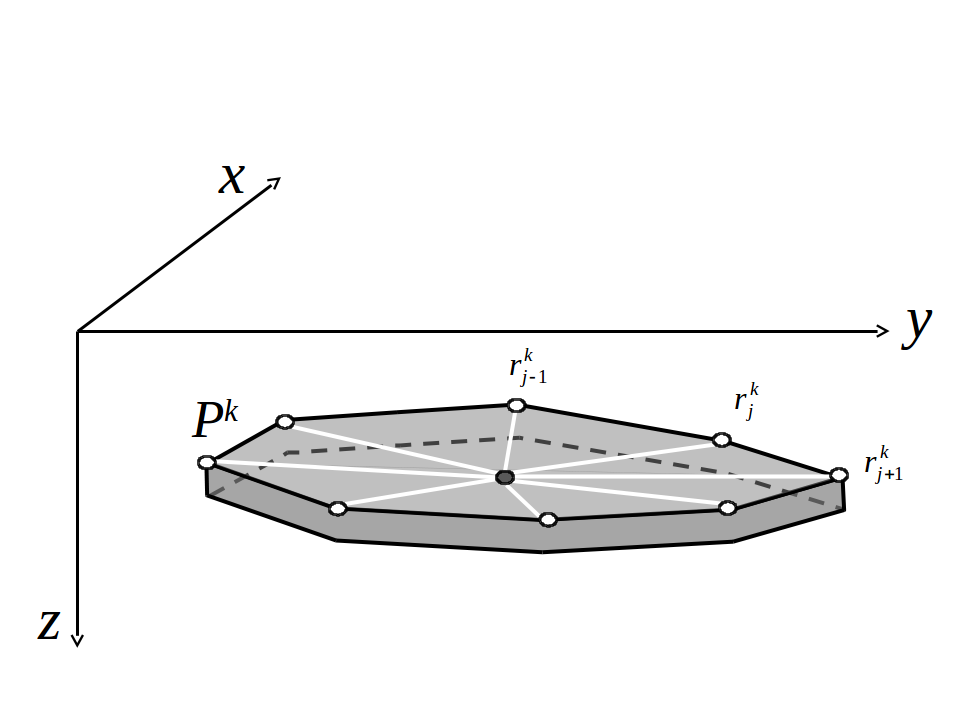
\includegraphics[scale=0.45]{Constraint_phi6.png}
	\caption{Representação esquemática do vínculo de Tikhonov de ordem zero nas distâncias radiais de um prisma $\varphi_{4}$. A figura exibe os prisma $P^k$ e suas respectivas distâncias radiais $r_j^k$ referidas à origem $O^k$. O vínculo atua sobre as distâncias radiais do prismas, levando-as próximas a zero.}
	\label{fig:phi4}
\end{figure}

Esse vínculo foi proposto por \cite{oliveirajr_etal2011} e \cite{oliveirajr_barbosa2013} e pode ser reescrito como
\begin{equation}\label{eq:phi4}
\begin{split}
\varphi_{4}(\mathbf{p}) &= \sum\limits^{L}_{k=1}\sum\limits^{V}_{j=1}\left(r_{j}^{k}\right)^2 \\
&= \mathbf{p}^{\mathsf{T}} \mathbf{R}_{4}^{\mathsf{T}} \mathbf{R}_{4} \mathbf{p}
\end{split} \quad ,
\end{equation}
em que
\begin{equation}
\mathbf{R}_{4} = 
\begin{bmatrix}
\mathbf{S}_{4} & \mathbf{0}_{(M-1) \times 1} \\
\mathbf{0}_{1 \times (M-1)} & 0 \\
\end{bmatrix}_{M\times M} \quad ,
\label{eq:R4-matrix}
\end{equation}
e
\begin{equation}
\mathbf{S}_{4} = 
\begin{bmatrix}
\mathbf{I}_{V} & \mathbf{0}_{V \times 2} \\
\mathbf{0}_{2 \times V} & \mathbf{I}_{2} \\
\end{bmatrix}_{ (V+2)\times (V+2)} \quad .
\label{eq:S4-matrix}
\end{equation}
O vetor gradiente e a matriz Hessiana da função $\varphi_{4}(\mathbf{p})$ (Equação \ref{eq:phi4}) são:
\begin{equation}\label{eq:phi4_gh}
\begin{split}
\boldsymbol{\nabla}\varphi_{4}(\mathbf{p}) &= 2\mathbf{R}^\mathsf{T}_{4}\mathbf{R}_{4}\mathbf{p} \quad ,\\
\mathbf{H}_{4}(\mathbf{p}) &= 2\mathbf{R}^\mathsf{T}_{4}\mathbf{R}_{4} \quad .
\end{split}
\end{equation}

Finalmente, o último vínculo é a \textit{norma Euclidiana mínima da espessura}, que impõe que a espessura comum $ dz $ de todos os prismas seja próxima de zero. Esse vínculo força que a profundidade da base do modelo seja o mais rasa possível (Figura \ref{fig:phi5})

%FIGURA
\begin{figure}[!htb]
	\centering
	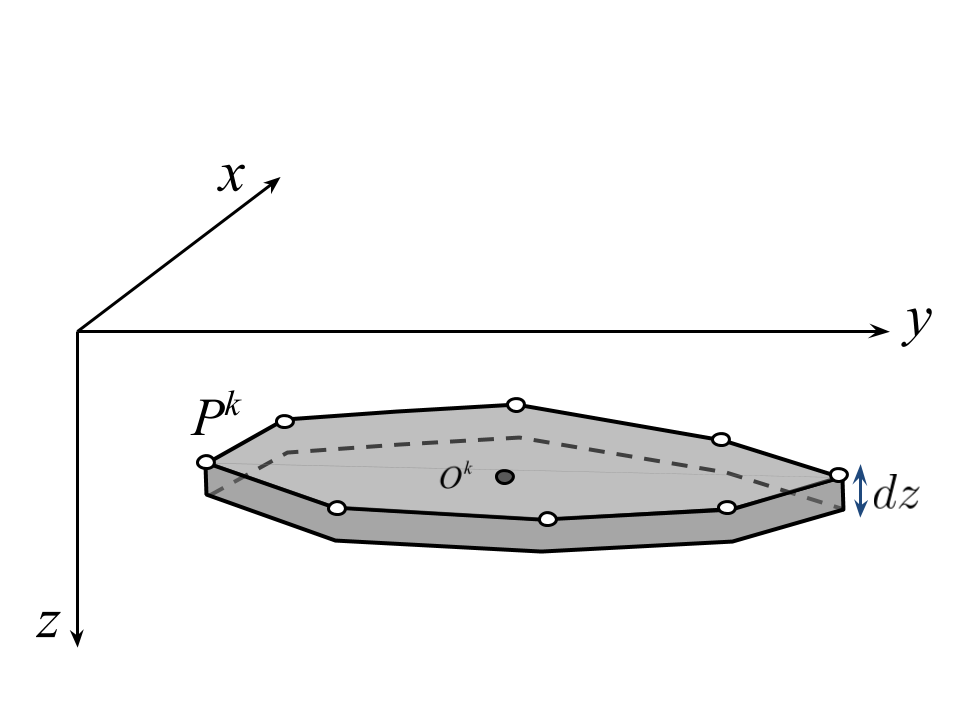
\includegraphics[scale=0.35]{Constraint_phi7.png}
	\caption{Representação esquemática do vínculo de Tikhonov de ordem zero $\varphi_{5}$ na espessura $dz$ dos prismas. A figura exibe os prisma $P^k$ e sua espessura. O vínculo atua sobre a espessura de os todos prismas levando-a próxima a zero, uma vez que $dz$ é igual para todos os prismas.}
	\label{fig:phi5}
\end{figure}

Esse vínculo pode ser escrito matematicamente como
\begin{equation}\label{eq:phi5}
\begin{split}
\varphi_{5}(\mathbf{p}) &= dz^2 \\
&= \mathbf{p}^{\mathsf{T}} \mathbf{R}_{5}^{\mathsf{T}} \mathbf{R}_{5} \mathbf{p}
\end{split} \quad ,
\end{equation}
em que
\begin{equation}
\mathbf{R}_{5} =
\begin{bmatrix}
\mathbf{0}_{(M-1) \times (M-1)} & \mathbf{0}_{(M-1) \times 1} \\
\mathbf{0}_{1 \times (M-1)} & 1 \\
\end{bmatrix}_{ M \times M } \quad .
\end{equation}
O vetor gradiente e a matriz Hessiana da função $\varphi_{5}(\mathbf{p})$ (Equação \ref{eq:phi5}) são:
\begin{equation}\label{eq:phi5_gh}
\begin{split}
\boldsymbol{\nabla}\varphi_{5}(\mathbf{p}) &= 2\mathbf{R}^\mathsf{T}_{5}\mathbf{R}_{5}\mathbf{p} \quad ,\\
\mathbf{H}_{5}(\mathbf{p}) &= 2\mathbf{R}^\mathsf{T}_{5}\mathbf{R}_{5} \quad .
\end{split}
\end{equation}

\section{Algoritmo de inversão}

Dada uma profundidade do topo do prisma mais raso $z_{0}$, a intensidade de magnetização total $m_{0}$ de todos os prismas, uma aproximação inicial $\hat{\mathbf{p}}_{(0)}$ para o vetor de parâmetros $\mathbf{p}$ (Equação \ref{eq:p-vector}), e os limites 
$p_{l}^{min}$ e $p_{l}^{max}$ (Equação \ref{eq:inequality-constraints}), o método de Levenberg-Marquardt \cite[por exemplo, ][ p. 624]{seber_wild2003} é utilizado para estimar o vetor de parâmetros $\hat{\mathbf{p}}^{\ast}$ que minimiza a função objetivo $\Gamma (\mathbf{p})$ (Equação \ref{eq:gamma}), sujeita aos vínculos de desigualdade definidos pela Equação \ref{eq:inequality-constraints}.
Para incorporar esses vínculos de desigualdade, foi empregada a mesma abordagem apresentada por \cite{barbosa_etal1999}, \cite{oliveirajr_etal2011} e \cite{oliveirajr_barbosa2013}.
Abaixo, segue o algoritmo de inversão aqui proposto:

\begin{itemize}
	\item[\textbf{entrada}] $\mathbf{d}^{o}$, $D_{0}$, $I_{0}$, $z_{0}$, 
	$m_{0}$, $D$, $I$, $p_{l}^{min}$ e $p_{l}^{max}$ (Equação 
	\ref{eq:inequality-constraints}), $k = 0$, $\hat{\mathbf{p}}_{(k)}$, e
	$\mathbf{W}_{(k)} = \mathbf{I}$, em que $\mathbf{I}$ é a matriz identidade de ordem $M$.
	\item[\textbf{(1)}] Computa a matriz $N \times M$ $\mathbf{G}(\hat{\mathbf{p}}_{(k)})$, cujo elemento $ij$ é a derivada do dado $d_{i}(\hat{\mathbf{p}}_{(k)})$ 
	(Equação \ref{eq:predicted-data-i}) com respeito ao $j$-ésimo elemento $p_{j}$ do vetor de parâme\-tros $\mathbf{p}$ (Equação \ref{eq:p-vector}):
	$$
	g_{ij} =  \dfrac{\partial d_{i}(\hat{\mathbf{p}}_{(k)})}{\partial{p_j}} \: .
	$$
	\item[\textbf{(2)}] Computa o vetor gradiente 
	$$
	\boldsymbol{\nabla} \phi(\hat{\mathbf{p}}_{(k)}) = 
	- \frac{2}{N} \mathbf{G}(\hat{\mathbf{p}}_{(k)})^{\top} 
	\mathbf{W}_{(k)} 
	\left[ \mathbf{d}^{o} - \mathbf{d}(\hat{\mathbf{p}}_{(k)}) \right]
	$$
	e a matriz Hessiana
	$$
	\mathbf{H}_{\phi}(\hat{\mathbf{p}}_{(k)}) = \frac{2}{N} 
	\mathbf{G}(\hat{\mathbf{p}}_{(k)})^{\top} \mathbf{W}_{(k)} 
	\mathbf{G}(\hat{\mathbf{p}}_{(k)})
	$$
	da função \textit{data-misfit} $\phi (\mathbf{p})$ (Equação \ref{eq:L2_misfit}),
	quando $\mathbf{W}_{(k)} = \mathbf{I}$, ou $\phi (\mathbf{p})$ 
	(Equação \ref{eq:L1_misfit}), quando $\mathbf{W}_{(k)} \ne \mathbf{I}$.
	Na próxima seção, será discutido como usar a matriz Hessiana 
	$\mathbf{H}_{\phi}(\hat{\mathbf{p}}_{(0)})$ (computada na iteração $k = 0$) 
	para definir os pesos $\alpha_{\ell}$ (Equação \ref{eq:gamma}) das funções de vínculos $\varphi_{\ell}(\mathbf{p})$ 
	(Equações \ref{eq:phi1}, \ref{eq:phi2}, \ref{eq:phi3}, \ref{eq:phi4} e \ref{eq:phi5}).
	\item[\textbf{(3)}] Computa o vetor gradiente 
	$$
	\boldsymbol{\nabla}\Gamma(\hat{\mathbf{p}}_{(k)}) = 
	\boldsymbol{\nabla}\phi (\hat{\mathbf{p}}_{(k)}) + 
	\sum\limits^{5}_{\ell =1} \alpha_{\ell} \, \boldsymbol{\nabla}\varphi_{\ell}(\hat{\mathbf{p}}_{(k)}) 
	$$ 
	e a matriz Hessiana
	$$
	\mathbf{H}(\hat{\mathbf{p}}_{(k)}) = 
	\mathbf{H}_\phi (\hat{\mathbf{p}}_{(k)}) + \sum\limits^{5}_{\ell =1} \alpha_{\ell} 
	\, \mathbf{H}_{\ell}
	$$ 
	da função objetivo $\Gamma (\mathbf{p})$ (Equação \ref{eq:gamma}),
	em que $\boldsymbol{\nabla}\varphi_{\ell}(\hat{\mathbf{p}}_{(k)})$ e
	$\mathbf{H}_{\ell}$ são, respectivamente, o vetor gradiente e a matriz Hessiana (Equações \ref{eq:phi1_gh}, \ref{eq:phi2_gh}, \ref{eq:phi3_gh}, \ref{eq:phi4_gh} e \ref{eq:phi5_gh}) das funções dos vínculos $\varphi_{\ell}(\mathbf{p})$ (Equações \ref{eq:phi1}, \ref{eq:phi2}, \ref{eq:phi3}, \ref{eq:phi4} e \ref{eq:phi5}).	
	\item[\textbf{(4)}] Computa o $l$-ésimo elemento $\hat{p}^{\dagger}_{l}$ de um vetor $\hat{\mathbf{p}}^{\dagger}_{(k)}$ como:
	$$
	\hat{p}^{\dagger}_{l} = -\ln\left(\frac{p_{l}^{max} - \hat{p}_{l}}{\hat{p}_{l} - p_{l}^{min}}\right) \: ,
	$$
	em que $\hat{p}_{l}$ é o $l$-ésimo elemento de $\hat{\mathbf{p}}_{(k)}$.
	\item[\textbf{(5)}] Computa uma matriz diagonal $\mathbf{T}(\hat{\mathbf{p}}_{(k)})$ 
	com o elemento $t_{ll}$ dado por
	$$
	t_{ll}(\hat{p}_{l}) = \frac{(p_{l}^{max} - \hat{p}_{l})(\hat{p}_{l} - p_{l}^{min})}{p_{l}^{max} - p_{l}^{min}} \: ,
	$$
	em que $p_{l}$ é o $l$-ésimo elemento do vetor $\hat{\mathbf{p}}_{(k)}$.
	\item[\textbf{(6)}] Computa uma matriz 
	$$
	\mathbf{H}^{\dagger}(\hat{\mathbf{p}}_{(k)}) = \mathbf{H}(\hat{\mathbf{p}}_{(k)})\mathbf{T}(\hat{\mathbf{p}}_{(k)}) \: .
	$$
	\item[\textbf{(7)}] Computa uma matriz diagonal $\mathbf{Q}_{(k)}$ com elemento $q_{ll}$ dado por 
	$$
	q_{ll} = \frac{1}{\sqrt{h^{\dagger}_{ll}}} \: ,
	$$
	em que $h^{\dagger}_{ll}$ é o elemento $ll$ da matriz $\mathbf{H}^{\dagger}(\hat{\mathbf{p}}_{(k)})$ .
	\item[\textbf{(8)}] Computa uma correção 
	$\boldsymbol{\Delta}\hat{\mathbf{p}}^{\dagger}_{(k)}$ para o vetor 
	$\hat{\mathbf{p}}^{\dagger}_{(k)}$ pela solução do sistema linear
	$$
	\mathbf{Q}_{(k)}^{-1} \left[ \mathbf{Q}_{(k)} 
	\mathbf{H}^{\dagger}(\hat{\mathbf{p}}_{(k)}) \mathbf{Q}_{(k)} + 
	\lambda_{(k)} \mathbf{I}_{M} \right] \mathbf{Q}_{(k)}^{-1}
	\boldsymbol{\Delta} \hat{\mathbf{p}}^{\dagger}_{(k)} = 
	- \boldsymbol{\nabla}\Gamma(\hat{\mathbf{p}}_{(k)}) \: ,
	$$
	%	$$
	%	\left[ \mathbf{H}^{\dagger}(\hat{\mathbf{p}}_{(k)}) + 
	%	\lambda_{(k)} \mathbf{D}_{(k)} \right] \boldsymbol{\Delta} \hat{\mathbf{p}}^{\dagger}_{(k)} = 
	%	- \boldsymbol{\nabla}\Gamma(\hat{\mathbf{p}}_{(k)}) \: ,
	%	$$
	em que $\lambda_{(k)}$ é um escalar positivo ajustado à cada iteração
	%	and $\mathbf{D}_{(k)}$ is a diagonal matrix formed by the diagonal elements 
	%	of $\mathbf{H}^{\dagger}(\hat{\mathbf{p}}_{(k)})$
	\citep[por exemplo,][p. 624]{seber_wild2003}.
	\item[\textbf{(9)}] Computa um novo vetor 
	%	\item[\textbf{(8)}] Compute a new vector 
	$$
	\hat{\mathbf{p}}^{\dagger}_{(k+1)} = \hat{\mathbf{p}}^{\dagger}_{(k)} + \boldsymbol{\Delta}\hat{\mathbf{p}}^{\dagger}_{(k)} \: .
	$$
	\item[\textbf{(10)}] Computa o $l$-ésimo elemento $ \hat{p}_{l} $ do novo vetor
	%	\item[\textbf{(9)}] Compute the $l$th element of the new vector 
	$\hat{\mathbf{p}}_{(k+1)}$ como:
	$$
	\hat{p}_{l} = p_{l}^{min} + \left(\frac{p_{l}^{max} - p_{l}^{min}}{ 1 + e^{-\hat{p}^{\dagger}_{l}} }\right) \: .
	$$
	\item[\textbf{(11)}] Se o seguinte critério de convergência for satisfeito,
	%	\item[\textbf{(10)}] If the following convergence criterion is satisfied,
	$$
	\Bigg|
	\frac{\Gamma(\hat{\mathbf{p}}_{(k+1)}) - \Gamma(\hat{\mathbf{p}}_{(k)})}
	{\Gamma(\hat{\mathbf{p}}_{(k)})} 
	\Bigg| \le \tau \: ,
	$$ 
	em que $\tau$ é um número positivo pequeno, que varia de $\approx 10^{-3}$ a 
	$10^{-4}$, que controla a convergência, o vetor de parâmetros $\hat{\mathbf{p}}_{(k+1)}$ é a solução. 
	Senão, atualiza o vetor de parâmetros 
	$$
	\hat{\mathbf{p}}_{(k)} \leftarrow \hat{\mathbf{p}}_{(k+1)} \: ,
	$$
	atualiza o elemento $ii$ da matriz $\mathbf{W}_{(k)}$
	$$
	w_{ii} = \frac{1}{\mid d_{i}^{o} -d_{i}(\hat{\mathbf{p}}_{(k)}) \mid + 
		\, \varepsilon} \: ,
	$$
	em que $\varepsilon$ possui um valor positivo pequeno ($\approx 10^{-10}$) usado
	para prevenir uma divisão por zero, atualiza o contador da iteração $k$
	$$
	k \leftarrow k + 1 \: ,
	$$
	e retorna à etapa (1).
\end{itemize}

Neste algoritmo, os elementos da matriz $\mathbf{G}(\hat{\mathbf{p}}_{(k)})$ 
(etapa 1) são computados pelo uso das diferenças finitas centradas.
É importante notar que na etapa 3 as matrizes Hessianas $\mathbf{H}_{\ell}$ (Equações \ref{eq:phi1_gh}, \ref{eq:phi2_gh}, \ref{eq:phi3_gh}, \ref{eq:phi4_gh} e \ref{eq:phi5_gh})
das funções dos vínculos $\varphi_{\ell}(\mathbf{p})$ 
(Equações \ref{eq:phi1}, \ref{eq:phi2}, \ref{eq:phi3}, \ref{eq:phi4} e \ref{eq:phi5}) 
não dependem do vetor de parâmetros. Por essa razão, eles são computados apenas uma vez antes da primeira iteração e armazenados para serem usados até a convergência ser alcançada (etapa 11).

Este algoritmo é executado para obter um corpo estimado para cada ponto 
$(m_{0}, z_{0})$ em uma malha de valores de profundidade do topo $z_{0}$ e intensidade de magnetização total $m_{0}$ definida pelo usuário. 
Todos os corpos estimados são obtidos através da utilização de uma aproximação inicial $\hat{\mathbf{p}}_{(0)}$ para o vetor de parâmetros
$\mathbf{p}$ (Equação \ref{eq:p-vector}), dos mesmos valores para os pesos
$\alpha_{\ell}$ (Equação \ref{eq:gamma}) e dos limites $p_{l}^{min}$ e 
$p_{l}^{max}$ (Eq. \ref{eq:inequality-constraints}) para os parâmetros estimados.
Os valores ótimos da profundidade do topo $z_{0}$ e intensidade de magnetização total
$m_{0}$ são escolhidos como aqueles associados aos corpos estimados que produzem os menores valores da função objetivo $\Gamma (\mathbf{p})$ (Equação \ref{eq:gamma}).

Note que, ao manter a matriz $\mathbf{W}_{(k)}$ (etapa 2 e 10) igual à identidade ao longo das iterações, o corpo estimado minimiza a norma-2 quadrática dos resíduos entro os dados observados e preditos (Equação \ref{eq:L2_misfit}). 
Nesse caso, o corpo estimado é a solução L2. 
A atualização iterativa dos elementos da matriz $\mathbf{W}_{(k)}$ com os valores absolutos dos resíduos de acordo com a etapa 10 é feita através do método IRLS \citep[][p. 46]{scales_gersztenkorn1988, aster_etal2019} para obter um corpo estimado que minimiza a norma-1 dos resíduos entre os dados observados e preditos 
(Equação \ref{eq:L1_misfit}). Nesse caso, o corpo estimado é a solução L1.

\section{Considerações práticas}

Nesta seção serão apresentados alguns aspectos práticos de como definir o conjunto de valores de profundidade do topo do prisma mais raso $z_{0}$, a intensidade de magnetização total $m_{0}$, a aproximação inicial
$\hat{\mathbf{p}}_{(0)}$ para o vetor de parâmetros $\mathbf{p}$ (Equação \ref{eq:p-vector}),
os pesos $\alpha_{\ell}$ (Equação \ref{eq:gamma}) das funções de vínculos 
$\varphi_{\ell}(\mathbf{p})$ 
(Equações \ref{eq:phi1}, \ref{eq:phi2}, \ref{eq:phi3}, \ref{eq:phi4} e \ref{eq:phi5}) e os limites $p_{l}^{min}$ e $p_{l}^{max}$ dos vínculos de desigualdade (Equação 
\ref{eq:inequality-constraints}).

Inicialmente, calcula-se a redução ao polo da anomalia de campo total observada. Essa é uma etapa dupla: ele permite a verificação dos valores usados para a direção de magnetização total (declinação $D$ e inclinação $I$) e é utilizado para estimar as dimensões horizontais da fonte alvo.
Se a fonte alvo possui uma direção de magnetização uniforme com valores de declinação e inclinação próximos daqueles escolhidos para $D$ e $I$, a anomalia RTP é predominantemente positiva sobre a fonte alvo e decai a zero perto de seus limites laterais.
Através da anomalia RTP estimada pela camada equivalente, é possível definir os limites $p_{l}^{min}$ e $p_{l}^{max}$ (Figura \ref{fig:barreira}) dos vínculos de desigualdade (Equação \ref{eq:inequality-constraints}) e uma aproximação inicial cilíndrica $\hat{\mathbf{p}}_{(0)}$, isto é, todos os prismas que formam $\hat{\mathbf{p}}_{(0)}$ possuem os vértices definidos por uma mesma distância radial constante $r_{0}$ e a mesma origem $(x_{0}, y_{0})$.
Nesta etapa, os pesos são $\alpha_{\ell}$ (Equação \ref{eq:gamma}) estabelecidos iguais a zero e se define uma malha de valores para a profundidade do topo $z_{0}$, intensidade de magnetização total $m_{0}$ e espessura $dz$ que produz, sem grande rigor, um ajuste entre dados observados $\mathbf{d}^{o}$ e dados preditos $\mathbf{d}(\hat{\mathbf{p}}_{(0)})$.

\pagebreak

%FIGURA
\begin{figure}[!htb]
	\centering
	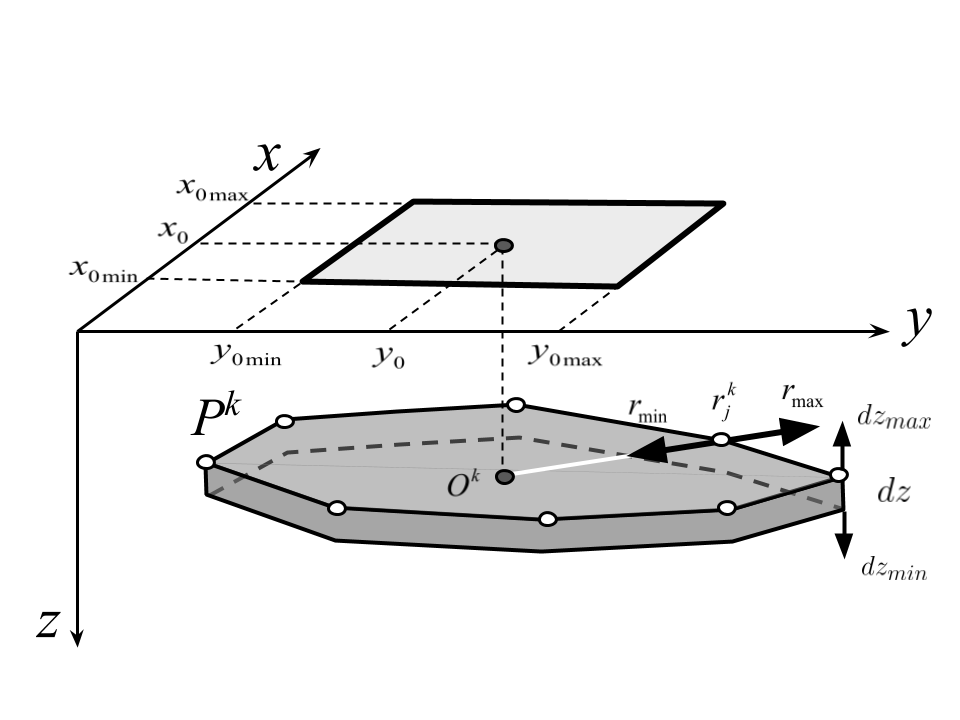
\includegraphics[width=0.75\linewidth]{Constraint_barrier.png}
	\caption{Representação esquemática dos vínculos de desigualdade. A figura exibe os prisma $P^k$ e os intervalos de máximo e mínimo de $r^k_j$, $x_0$, $y_0$ e $ dz $.}
	\label{fig:barreira}
\end{figure}

Um segundo aspecto crucial desse algoritmo consiste em definir os valores dos pesos $\alpha_{\ell}$ (Equação \ref{eq:gamma}). 
Não existe uma regra analítica para defini-los e seus valores podem depender das particularidades da área de estudo e do conjunto de dados observados.
Para contornar esse problema, os pesos $\alpha_{\ell}$ são definidos da seguinte maneira:
\begin{equation}\label{eq:alphas}
\alpha_{\ell} = \tilde{\alpha}_{\ell} \frac{E_{\phi}}{E_{\ell}}, 
\quad \ell = 1,\dots, 5 \: ,
\end{equation}
em que $\tilde{\alpha}_{\ell}$ é um escalar positivo e $ E_{\phi}/E_{\ell} $ 
é o fator de normalização.
Nessa equação, $E_{\ell}$ representa o traço da matriz Hessiana $\mathbf{H}_{\ell}$ (Equações \ref{eq:phi1_gh}, \ref{eq:phi2_gh}, \ref{eq:phi3_gh}, \ref{eq:phi4_gh} e \ref{eq:phi5_gh}) da $\ell$-ésima função de vínculo $\varphi_{\ell}(\mathbf{p})$
(Equações \ref{eq:phi1}, \ref{eq:phi2}, \ref{eq:phi3}, \ref{eq:phi4} e \ref{eq:phi5}).
A constante $E_{\phi}$ é o traço da matriz Hessiana
$\mathbf{H}_{\phi}(\hat{\mathbf{p}}_{(0)})$ (etapa 2 do algoritmo) da função \textit{data-misfit} $\phi(\mathbf{p})$ (Equação \ref{eq:L1_misfit}) computada na iteração
$k = 0$, com a aproximação inicial $\hat{\mathbf{p}}_{(0)}$ para o vetor de parâmetros $ \mathbf{p} $ (Equação \ref{eq:p-vector}).
Essa estratégia empírica permite definir indiretamente os pesos $\alpha_{\ell}$ 
(Equação \ref{eq:gamma}) pela utilização dos pesos normalizados $\tilde{\alpha}_{\ell}$ 
(Equação \ref{eq:alphas}), os quais dependem menos das características particulares do problema.
Baseado em experiência prática, os valores iniciais propostos aqui para os pesos normalizados $\tilde{\alpha}_{\ell}$ para ambas as funções \textit{data-misfit}, definidas pelas Equações \ref{eq:L2_misfit} e \ref{eq:L1_misfit}, são:
$\tilde{\alpha}_{1} = 10^{-4}$, $\tilde{\alpha}_{2} = 10^{-4}$, 
$\tilde{\alpha}_{3} = 10^{-4}$, $\tilde{\alpha}_{4} = 10^{-7}$, e 
$\tilde{\alpha}_{5} = 10^{-5}$.
Esses valores são comumente refinados de acordo com a informação a priori sobre a complexidade da fonte alvo. Por exemplo, ao aumentar ou diminuir valor de $\tilde{\alpha}_{1}$, força-se que o corpo estimado tenha fatias horizontais mais ou menos suaves; ao aumentar ou diminuir o valor de $\tilde{\alpha}_{3}$, força-se que o corpo estimado seja mais ou menos vertical. Os pesos normalizados
$\tilde{\alpha}_{1}$, $\tilde{\alpha}_{2}$, e $\tilde{\alpha}_{3}$ são comumente usados para introduzir informação a priori sobre o formato da fonte alvo. O peso normalizado $\tilde{\alpha}_{4}$ é geralmente usado como um parâmetro de regularização puramente matemático para obter soluções estáveis. Finalmente, o peso normalizado $\tilde{\alpha}_{5}$ é usualmente escolhido com o propósito de obter um corpo estimado com a profundidade da base mais rasa o possível.